81. \begin{figure}[ht!]
\center{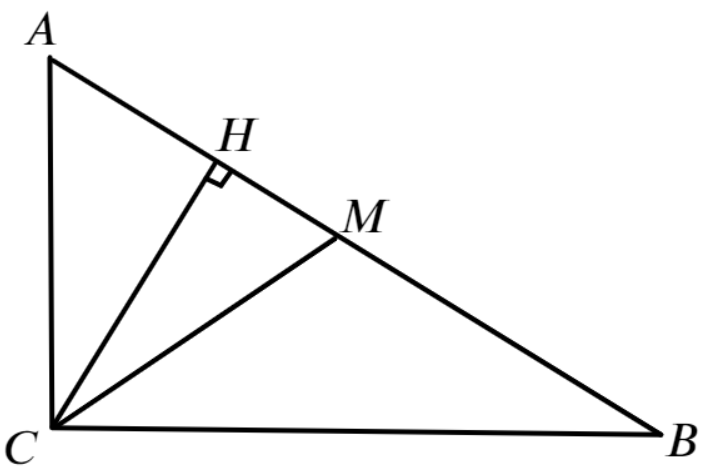
\includegraphics[scale=0.35]{g9-81.png}}
\end{figure}\\
Найдём $\angle B=90^\circ-53^\circ=37^\circ$ и $\angle ACH=90^\circ-53^\circ=37^\circ.$ Медиана, проведённая из прямого угла, равна половине гипотенузы, поэтому $CM=MB,$ а значит $\angle MCB=\angle B=37^\circ.$ Таким образом, $\angle HCM=90^\circ-37^\circ-37^\circ=16^\circ.$\\
